% '%' is similar to '//' in C++ to mean a single line comment. The LaTeX compiler will ignore these lines.

\documentclass[11pt]{article} % a back slash '\' denotes a command in LaTeX. The documentclass defines the standard layout of the document. Square brackets '[]' are parameters that can be passed to the argument.
\usepackage{amssymb,amsthm,listings,color,array,easytable,multicol} % packages like these bring in additional features via commands. They're like #include in C++
\usepackage[fleqn]{amsmath} % fleqn: flush left equations
\usepackage{venndiagram} % Here are a bunch more packages that I use frequently. Google them to find out what they are used for.
\usepackage{graphicx}
\usepackage{hyperref, url}
\usepackage[margin=2cm, top=2cm]{geometry}
\usepackage[shortlabels]{enumitem}
\graphicspath{{./img/}}
\newcommand\setItemNumber[1]{\setcounter{enumi}{\numexpr#1-1\relax}}
\newcommand*{\mybox}[1]{\framebox{#1}}
\newcommand{\tuple}[1]{$\langle #1 \rangle$} 
\newcommand{\stuple}[1]{$\langle$#1$\rangle$} % ordered pair with strings inside
\newcommand{\forceindent}{\leavevmode{\parindent=1em\indent}}

%The title, date, and author are part of the preamble. The preamble is not part of the main body of the document. 
\title{\bf Homework 6\\[1ex]
\rm\normalsize CS250 Discrete Structures I, Winter 2020 }
\date{\normalsize Due: May 10, 2020}
\author{\normalsize Armant Touche}

\begin{document} % This \begin{document} and corresponding \end{document} identifies the begeinning and end of your document body.

	\vspace{-4cm}\maketitle % \maketitle tells LaTeX to put the title, date, and author information here.
	
	\paragraph{Homework Exercises} Chapter 2: Sequences
	
	\subparagraph{Problem 1} 2.1 Describing Sequences (pg. 135-147)\\
			
		From section 2.1 in the textbook, complete exercises 2, 3, 7, 10, 13, 18

        \begin{enumerate}

            %2
            \setItemNumber{2}
            \item For each sequence given below, find a closed formula for $a_n$ , the $n$th term of the sequence (assume the first terms are $a_0$ ) by relating it to another sequence for which you already know the formula. In each case, briefly say how you got your answers.
                \begin{enumerate}
                    \item 4, 5, 7, 11, 19, 35, . . .
                    \item 0, 3, 8, 15, 24, 35,. . .
                    \item 6, 12, 20, 30, 42, . . .
                    \item 0, 2, 7, 15, 26, 40, 57, . . . (Cryptic Hint: these might be called “house numbers”)
                \end{enumerate}

            %3
            \item Write out the first 5 terms (starting with $a_0$ ) of each of the sequences described below. Then give either a closed formula or a recursive definition for the sequence (whichever is NOT given in the problem).
                \begin{enumerate}
                    \item $a_n = \frac{1}{2}(n^2 + n)$  
                    \item $a_n = 2a_{n - 1} - a_{n - 2}$ with $a_0 = 0$ and $a_1 = 1$
                    \item $a_n = na_{n - 1}$ with $a_0 = 1$
                \end{enumerate}

            %7
            \setItemNumber{7}
        \item Write out the first few terms of the sequence given by $a_1 = 3$; $a_n = 2a_{n - 1} + 4$. Then find a recursive definition for the sequence 10, 24, 52, 108, . . .


            %10
            \setItemNumber{10}
        \item Show that $a_n = 2^n - 5^n$ is also a solution to the recurrence relation $a_n  7a_{n − 1} − 10a_{n − 2}$. What would the initial conditions need to be for this to be the closed formula for the sequence?


            %13
            \setItemNumber{13}
        \item Use summation ($\Sigma$) or product ($\Pi$) notation to rewrite the following
            \begin{enumerate}

                \item $2 + 4 + 6 + 8 + ... + 2n$
                \item $1 + 5 + 9 + 13 + ... + 425$
                \item $1 + \frac{1}{2} + \frac{1}{3} + \frac{1}{4} + ... + \frac{1}{50}$
                \item $2\cdot 4\cdot 6\cdot ... \cdot2n$
                \item $(\frac{1}{2})(\frac{2}{3})(\frac{3}{4})...(\frac{100}{101})$
            \end{enumerate}

            %18
            \setItemNumber{18}
            \item When bees play chess, they use a hexagonal board like the one shown below. The queen bee can move one space at a time either directly to the right or angled up-right or down-right (but can never move leftwards). How many different paths can the queen take from the top left hexagon to the bottom right hexagon? Explain your answer, and this relates to the previous question. (As an example, there are three paths to get to the second hexagon on the bottom row.)

            \begin{center}
            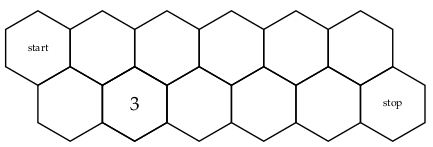
\includegraphics[width=.5\textwidth]{hw6_graphic1}
            \end{center}
	
        \end{enumerate}

	\subparagraph{Problem 2} 2.2 Arithmetic and Geometric Sequences (pg. 148-159)\\
	
		From section 2.2 in the textbook, complete exercises 1, 3, 4, 13, 15
	
        \begin{enumerate}

            %1
            \item Consider the sequence 5, 9, 13, 17, 21, . . . with $a_1 = 5$
                \begin{enumerate}

                \item Give a recursive definition for the sequence.
                \item Give a closed formula for the nth term of the sequence.
                \item Is 2013 a term in the sequence? Explain.
                \item How many terms does the sequence 5, 9, 13, 17, 21, . . . , 533 have?
                \item Find the sum: 5 + 9 + 13 + 17 + 21 + · · · + 533. Show your work.
                \item Use what you found above to find $b_n$ , the $n$th term of 1, 6, 15, 28, 45, . . ., where $b_0 = 1$
                \end{enumerate}


            %3
            \setItemNumber{3}
            \item Consider the sum 4 + 11 + 18 + 25 + · · · + 249.
                \begin{enumerate}
                    \item How many terms (summands) are in the sum?
                    \item Compute the sum using a technique discussed in this section.
                \end{enumerate}

            %4
            \item Consider the sequence 1, 7, 13, 19, . . . , $6n + 7$.
                \begin{enumerate}
                    \item How many terms are there in the sequence? Your answer will be in terms of $n$.
                    \item What is the second-to-last term?
                    \item Find the sum of all the terms in the sequence, in terms of n.
                \end{enumerate}


            %13
            \setItemNumber{13}
            \item If you have enough toothpicks, you can make a large triangular grid. Below, are the triangular grids of size 1 and of size 2. The size 1 grid requires 3 toothpicks, the size 2 grid requires 9 toothpicks.

            \begin{center}
            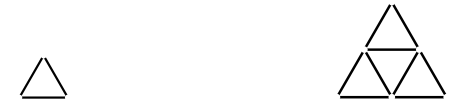
\includegraphics[width=.5\textwidth]{hw6_graphic2}
            \end{center}

                \begin{enumerate}
                    \item Let $t_n$ be the number of toothpicks required to make a size n triangular grid. Write out the first 5 terms of the sequence $t_1, t_2, ...$.
                    \item Find a recursive definition for the sequence. Explain why you are correct
                    \item Is the sequence arithmetic or geometric? If not, is it the sequence of partial sums of an arithmetic or geometric sequence? Explain why your answer is correct.
                    \item Use your results from part (c) to find a closed formula for the sequence. Show your work.
                \end{enumerate}

            %15
            \setItemNumber{15}
            \item Here is a surprising use of sequences to answer a counting question: How many license plates consist of 6 symbols, using only the three numerals 1, 2, and 3 and the four letters a, b, c, and d, so that no numeral appears after any letter? For example, “31ddac” and “12321” are acceptable license plates, but “13ba2c” is not.
                \begin{enumerate}
                    \item First answer this question by considering different cases: how many of the license plates contain no numerals? How many contain one numeral, etc.
                    \item Now use the techniques of this section to show why the answer is $4^7 - 3^7$.

                \end{enumerate}

        \end{enumerate}
	
	
		
\end{document}
